\batchmode
\makeatletter
\def\input@path{{/Users/Adam/Dropbox/Stat215A-2013/Labs/Lab2/Lab//}}
\makeatother
\documentclass[english]{article}\usepackage{graphicx, color}
%% maxwidth is the original width if it is less than linewidth
%% otherwise use linewidth (to make sure the graphics do not exceed the margin)
\makeatletter
\def\maxwidth{ %
  \ifdim\Gin@nat@width>\linewidth
    \linewidth
  \else
    \Gin@nat@width
  \fi
}
\makeatother

\IfFileExists{upquote.sty}{\usepackage{upquote}}{}
\definecolor{fgcolor}{rgb}{0.2, 0.2, 0.2}
\newcommand{\hlnumber}[1]{\textcolor[rgb]{0,0,0}{#1}}%
\newcommand{\hlfunctioncall}[1]{\textcolor[rgb]{0.501960784313725,0,0.329411764705882}{\textbf{#1}}}%
\newcommand{\hlstring}[1]{\textcolor[rgb]{0.6,0.6,1}{#1}}%
\newcommand{\hlkeyword}[1]{\textcolor[rgb]{0,0,0}{\textbf{#1}}}%
\newcommand{\hlargument}[1]{\textcolor[rgb]{0.690196078431373,0.250980392156863,0.0196078431372549}{#1}}%
\newcommand{\hlcomment}[1]{\textcolor[rgb]{0.180392156862745,0.6,0.341176470588235}{#1}}%
\newcommand{\hlroxygencomment}[1]{\textcolor[rgb]{0.43921568627451,0.47843137254902,0.701960784313725}{#1}}%
\newcommand{\hlformalargs}[1]{\textcolor[rgb]{0.690196078431373,0.250980392156863,0.0196078431372549}{#1}}%
\newcommand{\hleqformalargs}[1]{\textcolor[rgb]{0.690196078431373,0.250980392156863,0.0196078431372549}{#1}}%
\newcommand{\hlassignement}[1]{\textcolor[rgb]{0,0,0}{\textbf{#1}}}%
\newcommand{\hlpackage}[1]{\textcolor[rgb]{0.588235294117647,0.709803921568627,0.145098039215686}{#1}}%
\newcommand{\hlslot}[1]{\textit{#1}}%
\newcommand{\hlsymbol}[1]{\textcolor[rgb]{0,0,0}{#1}}%
\newcommand{\hlprompt}[1]{\textcolor[rgb]{0.2,0.2,0.2}{#1}}%

\usepackage{framed}
\makeatletter
\newenvironment{kframe}{%
 \def\at@end@of@kframe{}%
 \ifinner\ifhmode%
  \def\at@end@of@kframe{\end{minipage}}%
  \begin{minipage}{\columnwidth}%
 \fi\fi%
 \def\FrameCommand##1{\hskip\@totalleftmargin \hskip-\fboxsep
 \colorbox{shadecolor}{##1}\hskip-\fboxsep
     % There is no \\@totalrightmargin, so:
     \hskip-\linewidth \hskip-\@totalleftmargin \hskip\columnwidth}%
 \MakeFramed {\advance\hsize-\width
   \@totalleftmargin\z@ \linewidth\hsize
   \@setminipage}}%
 {\par\unskip\endMakeFramed%
 \at@end@of@kframe}
\makeatother

\definecolor{shadecolor}{rgb}{.97, .97, .97}
\definecolor{messagecolor}{rgb}{0, 0, 0}
\definecolor{warningcolor}{rgb}{1, 0, 1}
\definecolor{errorcolor}{rgb}{1, 0, 0}
\newenvironment{knitrout}{}{} % an empty environment to be redefined in TeX

\usepackage{alltt}
\usepackage[T1]{fontenc}
\usepackage[latin9]{inputenc}
\usepackage{geometry}
\geometry{verbose,tmargin=1in,bmargin=1in,lmargin=1in,rmargin=1in}
\usepackage{fancyhdr}
\pagestyle{fancy}
\setlength{\parskip}{\smallskipamount}
\setlength{\parindent}{0pt}
\usepackage{amsthm}
\usepackage{amsmath}

\makeatletter

%%%%%%%%%%%%%%%%%%%%%%%%%%%%%% LyX specific LaTeX commands.
\providecommand{\LyX}{L\kern-.1667em\lower.25em\hbox{Y}\kern-.125emX\@}

%%%%%%%%%%%%%%%%%%%%%%%%%%%%%% Textclass specific LaTeX commands.
\numberwithin{equation}{section}
\numberwithin{figure}{section}

\@ifundefined{date}{}{\date{}}
%%%%%%%%%%%%%%%%%%%%%%%%%%%%%% User specified LaTeX commands.
\pagestyle{empty} 

\makeatother

\usepackage{babel}
\begin{document}

\title{Lab 2 - Linguistic Survey\\
Stat 215A}


\author{Jonathan Fischer}
\date{October 7, 2014}

\maketitle


\section{Introduction}
In this report, we revisit the redwood data of Lab 1 to examine the effects of adding various smoothers to the temperature density and plots of temperature and humidity for a fixed time of day. For this exercise, we wish to observe the differences in performance among different kernel and parameter choices. 

The second element of the lab utilizes the lingual data collected by Bert Vaux in his 2003 Dialect Survey. In our treatment, we clean the data before examining a few questions geographically. To allow for better analysis, we convert the data from categorical responses to a sequence of 0's and 1's indicating the choices selected by respondents. This permits the use of PCA and subsequent K-means clustering based on projections to the principal axes. Optimal clustering seems to occur for K=3, and we observe groupings based in the northeast, south, and midwest/west. Perturbation by subsampling and different initial conditions for K-means produced identical clusters, engendering confidence in our results.

\section{Redwood Data}

\subsection{Temperature Density Estimates via Kernel Smoothing}

Our first task is to generate kernel density estimates of temperature based on the data obtained on the macroscope network. We used the cleaned data set from Lab 1 and aggregated over time and node id to get the entire temperature profile. Four kernels were considered for estimation--biweight, Epanechnikov, Gaussian, and rectangular. We examined the density estimates for five choices of the bandwidth, as shown in Figure 2.1. Smaller bandwidths produced excessively spiky densities, though an adjustment factor of 1 or greater mitigated this concern. The high bandwidths resulted in oversmoothing, more or less yielding gaussian distributions. This reflects the bias-variance tradeoff in which bandwidth positively correlates with bias but negatively correlates with variance (see Homework 2.) The smaller bandwidth estimators suggest a trimodal density with peaks at around 10, 15, and 20 degrees Celsius. All kernels performed similarly with the exception of the rectangular kernel, which gave unstable estimates highly dependent on the bandwidth. 

\begin{figure}
\begin{center}
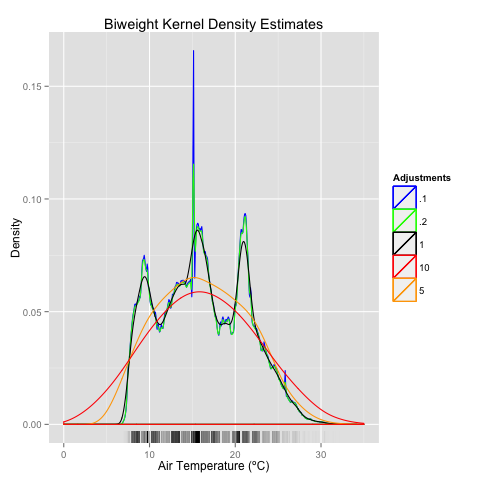
\includegraphics[scale = .4]{Temperature_Density_Biweight_Kernel.png}
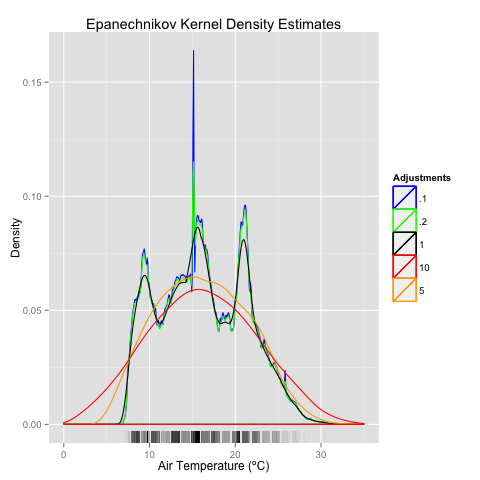
\includegraphics[scale = .4]{Temperature_Density_Epanechnikov_Kernel.png}
\end{center}

\begin{center}
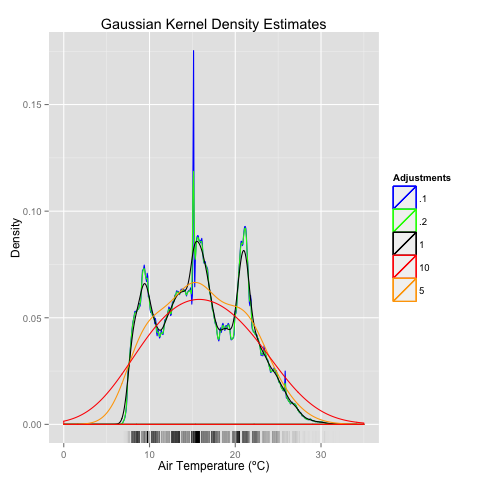
\includegraphics[scale = .4]{Temperature_Density_Guassian_Kernel.png}
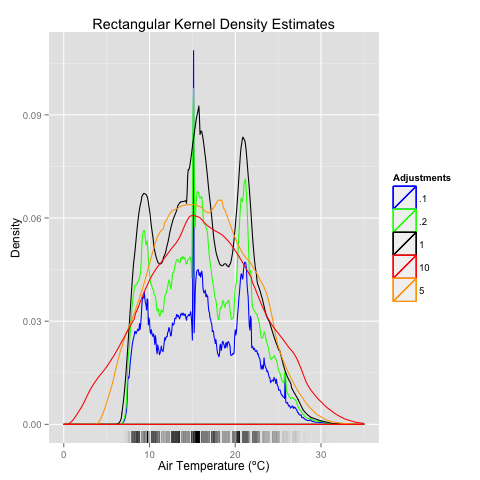
\includegraphics[scale = .4]{Temperature_Density_Rectangular_Kernel.png}
\end{center}
\caption{Kernel smoothed estimates of the temperature density for four different kernels. The rectangular kernel performs the worst while the others produce similar densities. Bandwidth = adjustment * .392 where .392 is the optimal bandwidth as calculated in R by bw.nrd0.}
\end{figure}

\subsection{Loess Smoothed Humidity vs Temperature}

To investigate Loess smoothing, we fixed the time of day at 10:05 AM and plotted humidity against temperature. We observe the negative correlation as before and fit Loess smoothers with polynomial degrees 0, 1, and 2 for four different spans. Here, the span is not an absolute bandwidth, rather it represents the proportion of points used in the smoother. For example, a span of .25 means we take the x closest points where x/n = .25 and n is the number of observations. Thus changing this value is akin to varying the bandwidth. Figure 2.2 shows the results. The degree 0 smoother does rather poorly compared to the higher degree versions as it is too flat for all spans. The degree 1 and 2 smoothers behave similarly, though the second-degree fit seems subtly more consistent across spans. As in the KDE plots, higher spans give a smoother trend while lower ones are more sensitive to the local behavior. 

\begin{figure}
\begin{center}
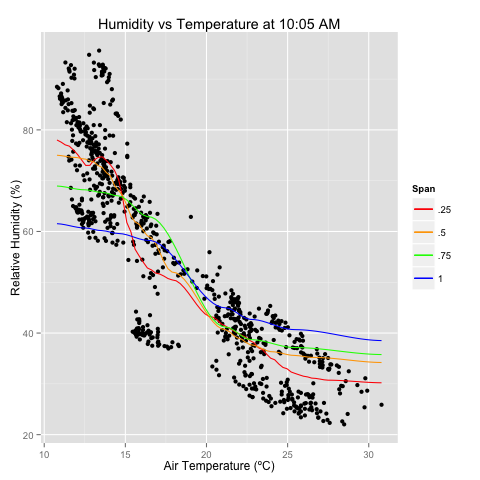
\includegraphics[scale = .4]{Humidity_Temperature_Loess_0.png}
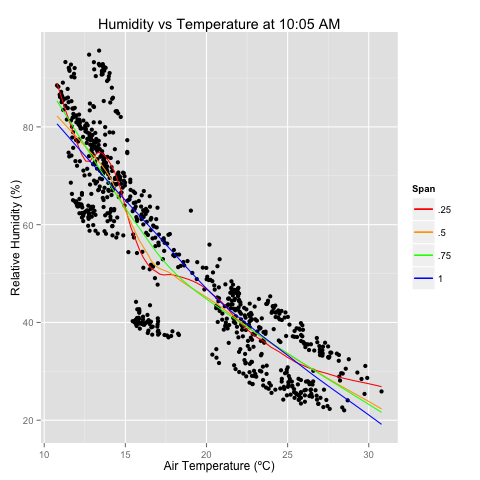
\includegraphics[scale = .4]{Humidity_Temperature_Loess_1.png}
\end{center}

\begin{center}
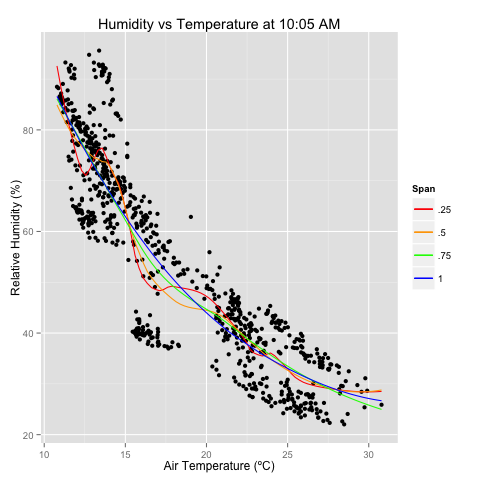
\includegraphics[scale = .4]{Humidity_Temperature_Loess_2.png}
\end{center}
\caption{Upper Left: Degree 0 Loess smoother. Upper right: Degree 1 Loess smoother. Bottom: Degree 2 Loess smoother. The second degree smoother produces more consisten results, but the degree one gives similar trends.}
\end{figure}



\section{Linguistic Data}


\subsection{Data quality and cleaning}

Each row of the data contains a participant's answers and each column corresponds to a different question. The entries are categorical variables that give the responses in the form of numbers where each number is associated with a specific answer. There were initially 47471 participants and 67 questions considered. Since we want to eventually generate maps using latitude and longitude, we began by removing all rows for which a latitude and longitude were not present. This was a total of 1020 respondents. Several systematic reasons for the missing coordinate data were considered, including zip codes starting with 0 and outdated zip code databases. Investigation of these possiblities yielded no improvement. Additionally, some participants answered few of the questions and were removed. We set a cutoff of 20 missing answers. This left us with 45107 observations. While they were included in the data for clustering, any points corresponding to locations in Alaska and Hawaii were removed for plotting. The latitude and longitude columns were separated from the response columns before encoding to binary variables since that procedure would not work if they remained. Furthermore, they were not readded until clustering was complete since PCA and the clusters would be influenced by the presence of location data and we would likely get geographic clusters by default.

Having the data in categorical form was sufficient for the EDA as it allowed for plotting and tracking how often responses were recorded together. However, further analysis required a transformation into binary variables as described in the lab's prompt. This was accomplished by defining a function based on model.matrix and applying it to each row of the data. The intercept columns were then removed to give a set of 468 binary response variables where a 0 indicates that answer was not chosen and a 1 says the opposite. 


\subsection{Exploratory Data Analysis}

Our EDA began with maps of the US overlaid with responses by latitude and longitude. Each point is colored by the responder's answer. For each question only the popular choices were included to prevent overplotting. The included plots correspond to the most important questions as measured by the loadings on the first 3 principal components. These are the plural second person, name for athletic shoes, and name for a water fountain questions. In Figure 3.1, the south is shown to strongly prefer using "y'all" while the rest of the nation favors "you", "you all", or "you guys" with no clear geographical trend among them. Figure 3.2 illustrates the divide in usage of "sneakers" and "tennis shoes." The northeast refers to the shoes in question as sneakers while the remainder of the country uses tennis shoes. In both examples, we see south Florida's behavior mimicking that of the northeast, perhaps as a consequence of the large number of transplants in the region. The final of our EDA plots, Figure 3.3, shows the geographic separation between the terms "water fountain" and "drinking fountain," with "drinking fountain" only being common in parts of the midwest and on the west coast. Considering these plots together, we note that each one defines a group. In fact, these correspond nicely to the clusters output by PCA and K-means. 

To look at the relationship between a pair of questions, we look at the second person plural and shoes questions. 
\begin{figure}
\begin{center}
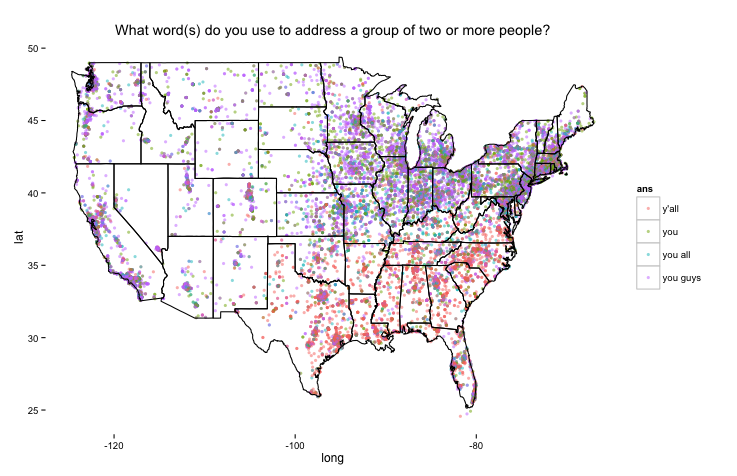
\includegraphics[scale = .5]{Rplot1.png}
\end{center}
\caption{Most popular ways to address a group of people mapped by latitude and longitude. Y'all is popular in the south, but the other choices are evenly spread across the rest of the country.}
\end{figure}

\begin{figure}
\begin{center}
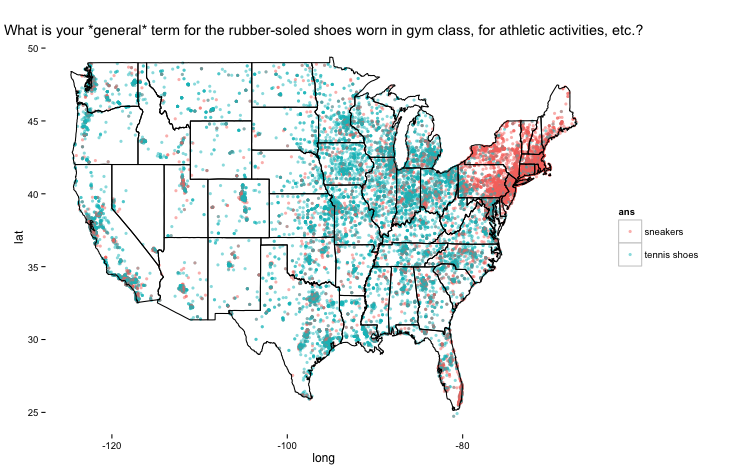
\includegraphics[scale = .5]{Rplot2.png}
\end{center}
\caption{Mapped responses for tennis shoes/sneakers. The northeast is the only region to prefer sneakers.}
\end{figure}

\begin{figure}
\begin{center}
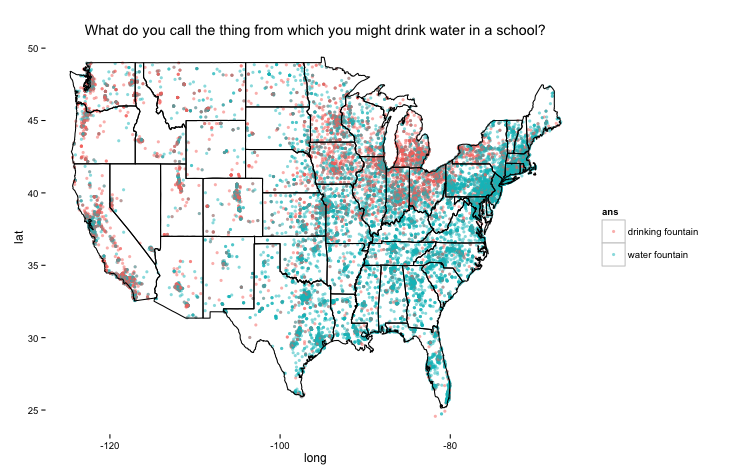
\includegraphics[scale = .5]{Rplot3.png}
\end{center}
\caption{Map of water/drinking fountain usage. The upper midwest and west coast show a preference for drinking fountain while everyone else says water fountain.}
\end{figure}



\section{Dimension reduction methods}

This is where you discuss and show plots about the results of whatever
dimension reduction techniques you tried - PCA, hierarchical clustering,
K-means, random projections, etc.

\begin{figure}
\begin{center}
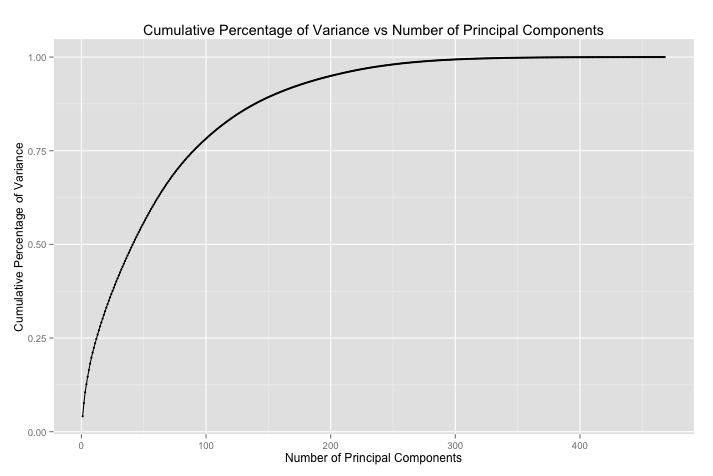
\includegraphics[scale=.3]{/Users/jonathanfischer/STAT215A/cumulativevariance.png}
\end{center}
\caption{Cumulative variance as a function of the number of principal components.}
\end{figure}

\begin{figure}
\begin{center}
\includegraphics[scale = .3]{PCA12bw.png}
\includegraphics[scale = .3]{PCA12c.png}
\end{center}
\caption{Scatter plot of projections onto the first and second principal component axes with and without annotation of K-means defined clusters.}
\end{figure}

\begin{figure}
\begin{center}
\includegraphics[scale = .3]{PCA13bw.png}
\includegraphics[scale = .3]{PCA13c.png}
\caption{Scatter plot of projections onto the first and third principal component axes with and without annotation of K-means defined clusters.}
\end{center}
\end{figure}

\begin{figure}
\begin{center}
\includegraphics[scale = .3]{PCA23bw.png}
\includegraphics[scale = .3]{PCA23c.png}
\end{center}
\caption{Scatter plot of projections onto the second and third principal component axes with and without annotation of K-means defined clusters.}
\end{figure}

\begin{figure}
\begin{center}
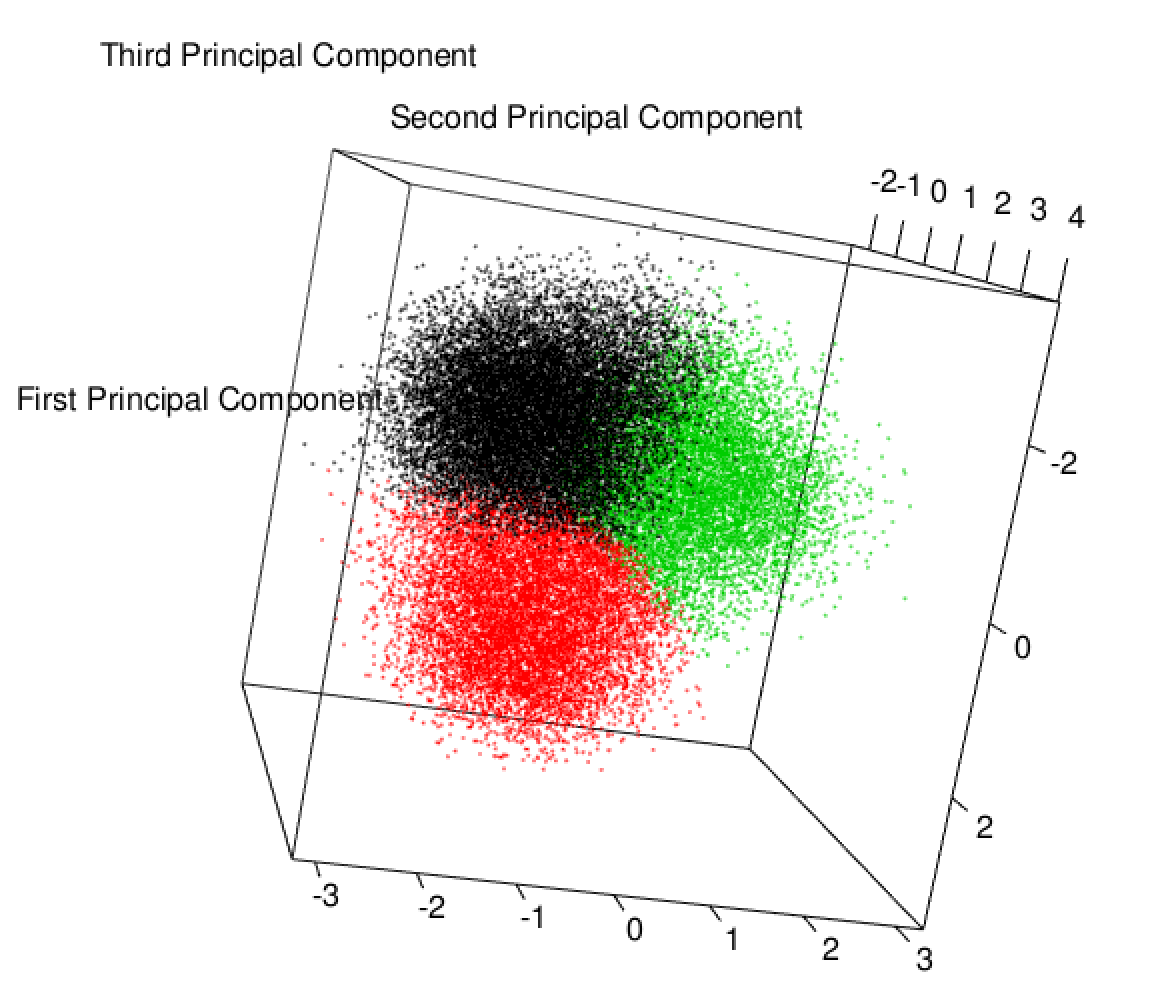
\includegraphics[scale = .4]{PCA3DScatter.png}
\caption{Screenshot of projection to first three principal axes with cluster coloring.}
\end{center}
\end{figure}

\begin{figure}
\begin{center}
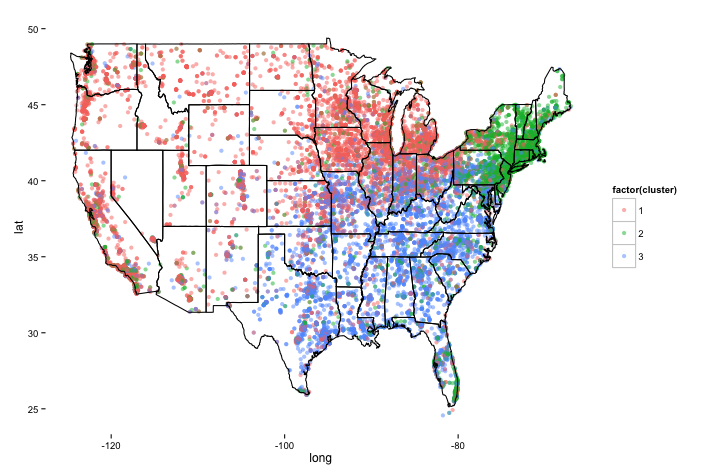
\includegraphics[scale=.5]{clusters.png}
\end{center}
\caption{Responders mapped onto USA and colored by K-means generated clusters with K=3. We see 3 geographically well-defined clusters--northeast, south, and midwest/west.}
\end{figure}

\begin{figure}
\begin{center}
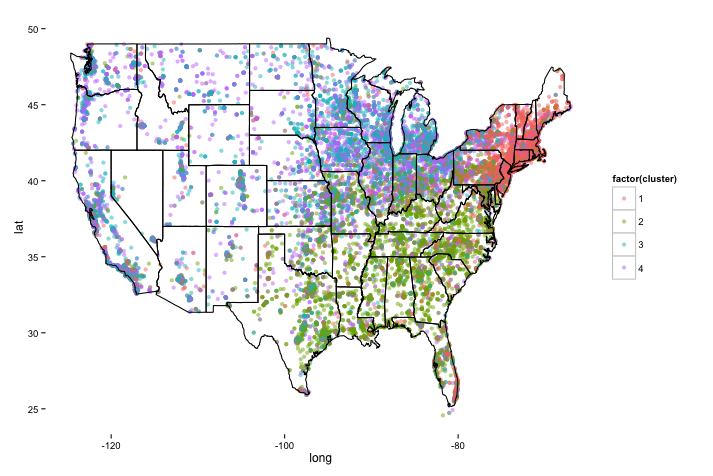
\includegraphics[scale=.5]{pcamap4clusters.png}
\end{center}
\caption{Responders mapped onto USA and colored by K-means generated clusters with K=4. The south and northeast clusters remain but two clusters are mixed throughout the west/midwest. This suggests 3 clusters was more appropriate.}
\end{figure}


\begin{verbatim}
http://youtu.be/-qgCEqmbsO4
http://youtu.be/FuRNZofyJgs
\end{verbatim}



\section{Stability of findings to perturbation}

\begin{figure}
\begin{center}
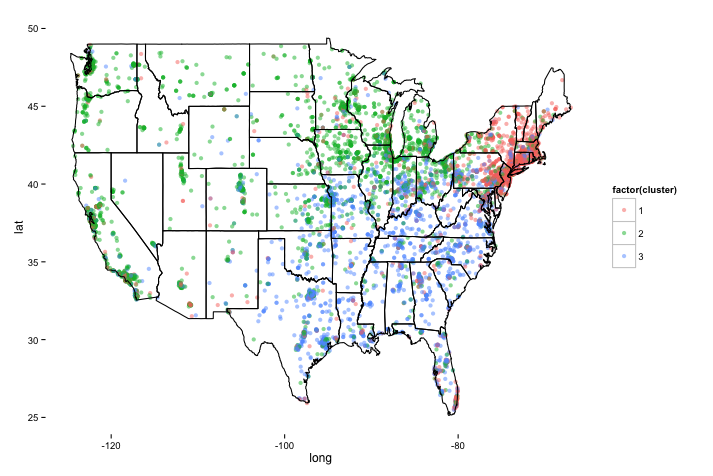
\includegraphics[scale=.5]{pcasubsample.png}
\end{center}
\caption{The results of PCA and clustering with K=3 with a random subsample of 10000 points. The same geographic clusters arise.}
\end{figure}

\begin{figure}
\begin{center}
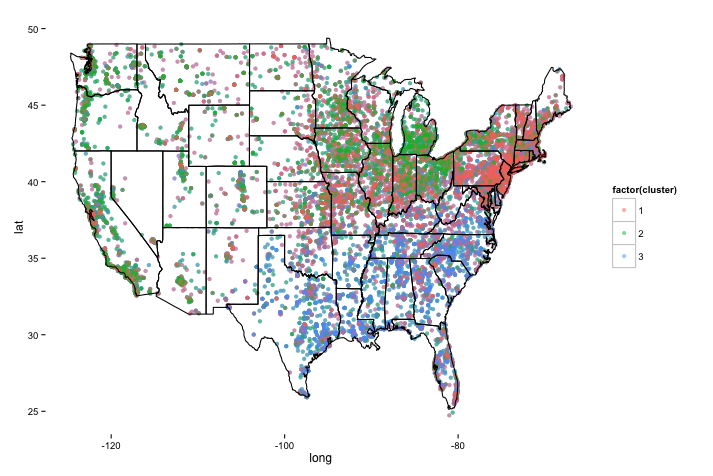
\includegraphics[scale=.5]{pca3questions.png}
\end{center}
\caption{The results of PCA and clustering with K=3 where the data have been reduced to responses to questions 50 (not y'all/y'all), 73 (sneakers/tennis shoes), and 103 (water/drinking fountain). There is more overlap in the clusters than when the full data are used, but we still see the distinct geographic pattern.}
\end{figure}


\section{Conclusion}
\end{document}
